%% This is file `elsarticle-template-1-num.tex',
%%
%% Copyright 2009 Elsevier Ltd
%%
%% This file is part of the 'Elsarticle Bundle'.
%% ---------------------------------------------
%%
%% It may be distributed under the conditions of the LaTeX Project Public
%% License, either version 1.2 of this license or (at your option) any
%% later version.  The latest version of this license is in
%%    http://www.latex-project.org/lppl.txt
%% and version 1.2 or later is part of all distributions of LaTeX
%% version 1999/12/01 or later.
%%
%% Template article for Elsevier's document class `elsarticle'
%% with numbered style bibliographic references
%%
%% $Id: elsarticle-template-1-num.tex 149 2009-10-08 05:01:15Z rishi $
%% $URL: http://lenova.river-valley.com/svn/elsbst/trunk/elsarticle-template-1-num.tex $
%%
\documentclass[12pt]{elsarticle}

%% Use the option review to obtain double line spacing
%% \documentclass[preprint,review,12pt]{elsarticle}

%% Use the options 1p,twocolumn; 3p; 3p,twocolumn; 5p; or 5p,twocolumn
%% for a journal layout:
%% \documentclass[final,1p,times]{elsarticle}
%% \documentclass[final,1p,times,twocolumn]{elsarticle}
%% \documentclass[final,3p,times]{elsarticle}
%% \documentclass[final,3p,times,twocolumn]{elsarticle}
%% \documentclass[final,5p,times]{elsarticle}
%% \documentclass[final,5p,times,twocolumn]{elsarticle}

%% The graphicx package provides the includegraphics command.
\usepackage{graphicx}
%% The amssymb package provides various useful mathematical symbols
\usepackage{amssymb}
\usepackage{comment}
\usepackage{amsmath}
\usepackage{blkarray}
\usepackage{listings}
\usepackage{subcaption}
\usepackage{amsmath}

%% The amsthm package provides extended theorem environments
%% \usepackage{amsthm}

%% The lineno packages adds line numbers. Start line numbering with
%% \begin{linenumbers}, end it with \end{linenumbers}. Or switch it on
%% for the whole article with \linenumbers after \end{frontmatter}.
\usepackage{lineno}

%% natbib.sty is loaded by default. However, natbib options can be
%% provided with \biboptions{...} command. Following options are
%% valid:

%%   round  -  round parentheses are used (default)
%%   square -  square brackets are used   [option]
%%   curly  -  curly braces are used      {option}
%%   angle  -  angle brackets are used    <option>
%%   semicolon  -  multiple citations separated by semi-colon
%%   colon  - same as semicolon, an earlier confusion
%%   comma  -  separated by comma
%%   numbers-  selects numerical citations
%%   super  -  numerical citations as superscripts
%%   sort   -  sorts multiple citations according to order in ref. list
%%   sort&compress   -  like sort, but also compresses numerical citations
%%   compress - compresses without sorting
%%
%% \biboptions{comma,round}

% \biboptions{}

\journal{ECS 132 Final Project}

\begin{document}

%% Title, authors and addresses

\title{ECS 132 Final Course Project}

%% use the tnoteref command within \title for footnotes;
%% use the tnotetext command for the associated footnote;
%% use the fnref command within \author or \address for footnotes;
%% use the fntext command for the associated footnote;
%% use the corref command within \author for corresponding author footnotes;
%% use the cortext command for the associated footnote;
%% use the ead command for the email address,
%% and the form \ead[url] for the home page:
%%
%% \title{Title\tnoteref{label1}}
%% \tnotetext[label1]{}
%% \author{Name\corref{cor1}\fnref{label2}}
%% \ead{email address}
%% \ead[url]{home page}
%% \fntext[label2]{}
%% \cortext[cor1]{}
%% \address{Address\fnref{label3}}
%% \fntext[label3]{}


%% use optional labels to link authors explicitly to addresses:
%% \author[label1,label2]{<author name>}
%% \address[label1]{<address>}
%% \address[label2]{<address>}

\author{Justin Jia, Ethan Wang, Ho Lun Sin, and Yangzihao Wang}

\address{\{bwjia,eycwang,hsin,yzhwang\}@ucdavis.edu}

\maketitle

%%\begin{keyword}
%% keywords here, in the form: keyword \sep keyword

%% MSC codes here, in the form: \MSC code \sep code
%% or \MSC[2008] code \sep code (2000 is the default)

%%\end{keyword}


%%
%% Start line numbering here if you want
%%

%% main text
\section{Problem A}
\label{PA}
We use users' average ratings as random samples to compute the approximate 95\% confidence
interval for: the population mean rating by men, by women, and the difference between the two means. We show the results in Table~\ref{tab1}.
\begin{table*}[ht]
\begin{tabular}{l*{2}{c}r}
                 & From & To \\
\hline
approx. CI for E(ratings by men) & 3.561174 & 3.616033 \\
approx. CI for E(ratings by women) & 3.556519 & 3.617838  \\
approx. CI for E(rating diffs by gender) & -0.03971356 & 0.04256391\\
\end{tabular}
\caption{Approximate 95\% confidence interval for various means.}
\label{tab1}
\end{table*}

From Table~\ref{tab1} we observe that the center of approximate 95\% confidence interval of the rating differences by gender is close to 0. Let the null hypothesis be that "the male and female population means are equal". We form a significance test of this hypothesis. We show the output of our significant test in the following code snapshot:
\begin{lstlisting}[language=R]
Two Sample t-test

data: a and b
t = 0.0446, df = 941, p-value = 0.9645
alternative hypothesis: true difference in means is not equal to 0
95 percent confidence interval:
 -0.06134628  0.06419663
sample estimates:
mean of x mean of y 
 3.588604  3.587179
\end{lstlisting}
The 0.9645 p-value shows no significant evidence to reject the null hypothesis, thus we should accept the hypothesis that the male and female population means are equal. Figure~\ref{fig1} further corroborates our conclusion.
\begin{figure}[h!]
\centering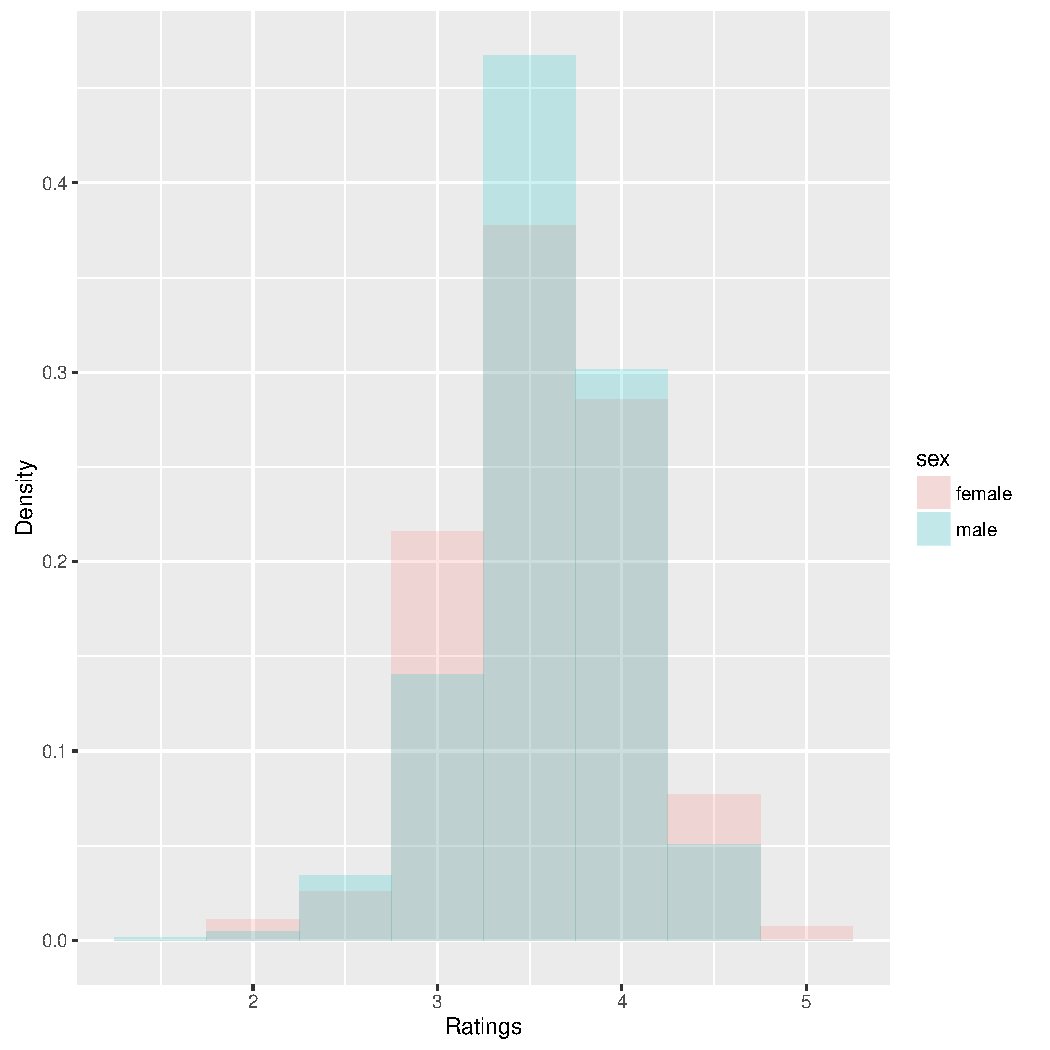
\includegraphics[width=0.45\textwidth]{ratings.pdf}
\caption{Histograms of the male and female ratings.}
\label{fig1}
\end{figure}

We show the approximate 95\% confidence interval for the difference between the population mean number of ratings by men and women, as well as the approximate 95\% confidence interval for the population proportion of users who are men in Table~\ref{tab2}
\begin{table*}[h]
\begin{tabular}{l*{2}{c}r}
                 & From & To \\
\hline
approx. CI for E(rating number diffs by gender) & 7.505438 & 25.59478\\
approx. CI for proportion of male users & 0.6815512 & 0.7394457 \\
\end{tabular}
\caption{Approximate 95\% confidence interval for mean diff and proportion.}
\label{tab2}
\end{table*}

We use a linear model to estimate the population regression function in which we predict rating from age and gender. The summary output is shown in the following code snapshot:
\begin{lstlisting}[language=R]
Call:
lm(formula = data$avg.rating ~ data$age + data$gender)

Residuals:
     Min       1Q   Median       3Q      Max 
-2.06903 -0.25972  0.03078  0.27967  1.34615 

Coefficients:
             Estimate Std. Error t value Pr(>|t|)    
(Intercept) 3.4725821  0.0482655  71.947  < 2e-16 ***
data$age    0.0033891  0.0011860   2.858  0.00436 ** 
data$gender 0.0002862  0.0318670   0.009  0.99284    
---
Signif. codes:  0 ‘***’ 0.001 ‘**’ 0.01 ‘*’ 0.05
‘.’ 0.1 ‘ ’ 1

Residual standard error: 0.4438 on 940 degrees of freedom
Multiple R-squared:  0.008615,	Adjusted R-squared:  0.006505 
F-statistic: 4.084 on 2 and 940 DF,  p-value: 0.01714
\end{lstlisting}
The confidence interval of $\beta_1$ (age coefficient) is from 0.001064581 to 0.01714. From the output of $summary(lmout)$ we observe that its p-value is 0.00436, which means the difference between null hypothesis ($\beta_1$ is 0) and our sample results is significant enough for us to reject the null hypothesis.

The approximate 95\% confidence interval for population mean rating of women of age 28 is from 3.513127 to 3.621827. We show the visualization of our linear model in Figure~\ref{fig2}.

\begin{figure}[h!]
\centering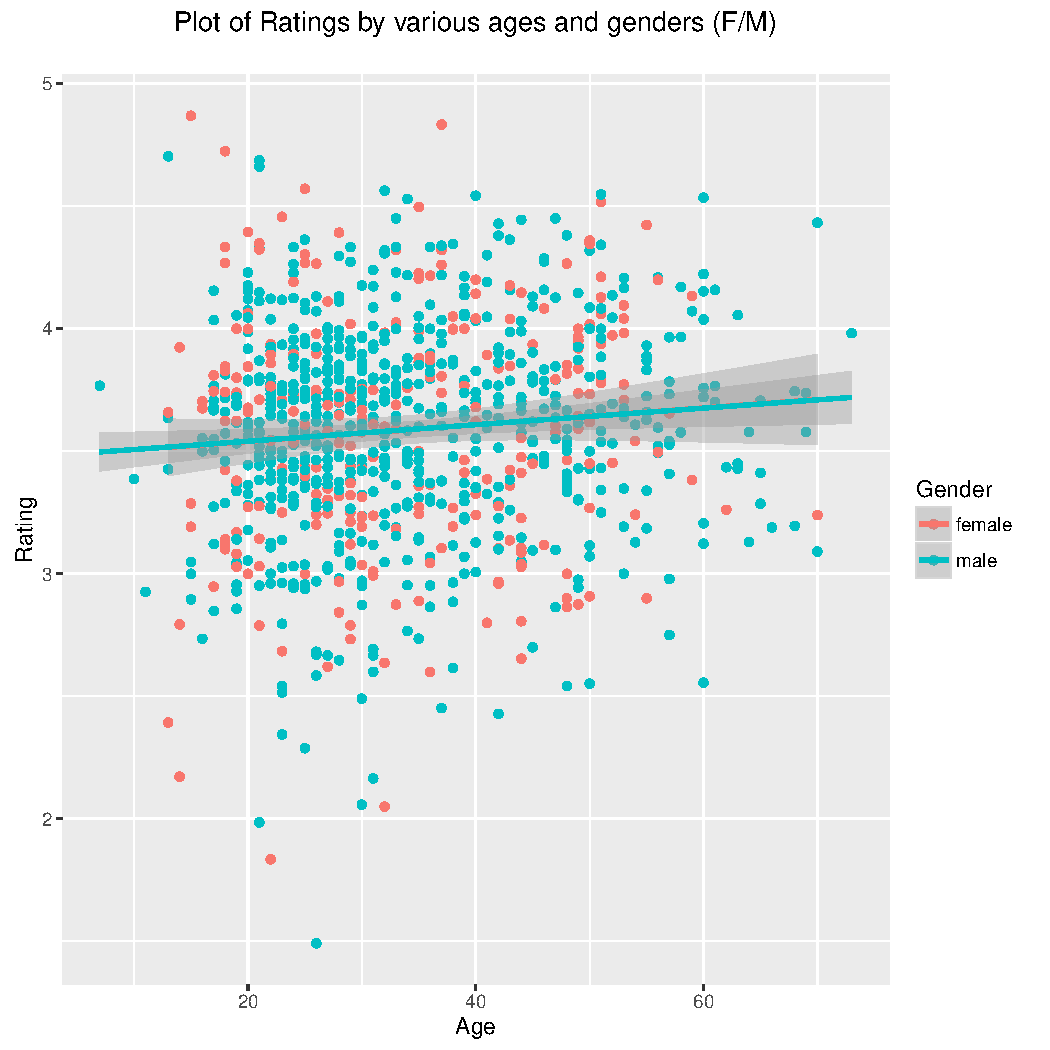
\includegraphics[width=0.45\textwidth]{predict.pdf}
\caption{Linear model of ratings and age and gender.}
\label{fig2}
\end{figure}

\section{Problem B}
\label{PB}
In this section we analyze the Wordbank dataset. More specifically, we form a linear regression model from a description point of view, by showing the relationship between vocabulary size and age (in months), birth order, ethnicity, sex and mon's education. Figure~\ref{fig:sfig1} shows the quantile of vocabulary size at different age. We observe a clear direct proportional relationship between age and vocabulary size. We also observe such relationship in Figure~\ref{fig:sfig2}, which shows the linear regression model of vocabulary size with age. It also reveals that female children have larger mean vocabulary size than male children, at all ages, regardless of other factors.

\begin{figure}
\begin{subfigure}{.5\textwidth}
  \centering
  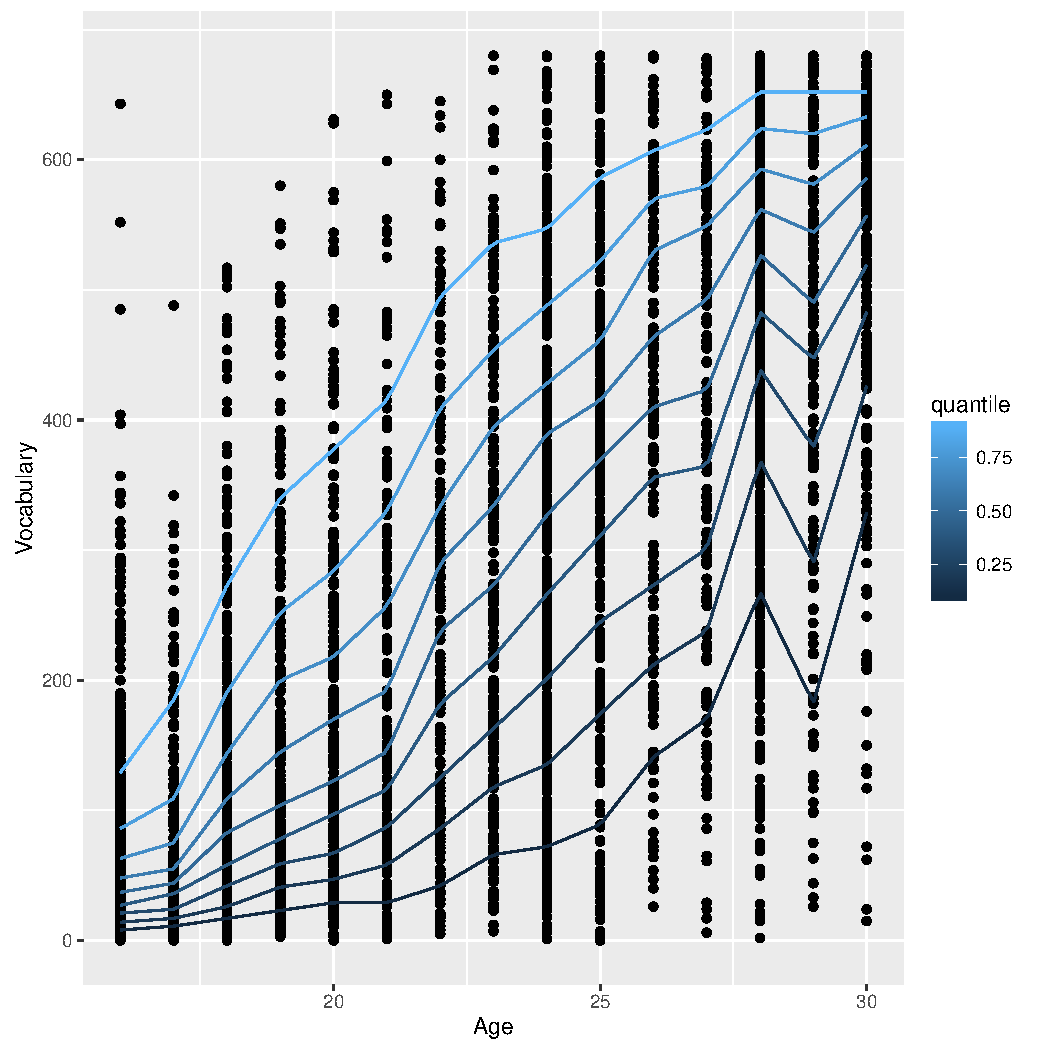
\includegraphics[width=.9\textwidth]{quantile-vocab-age.pdf}
  \caption{Quantile graph of vocabulary changes over age increase.}
  \label{fig:sfig1}
\end{subfigure}%
\begin{subfigure}{.5\textwidth}
  \centering
  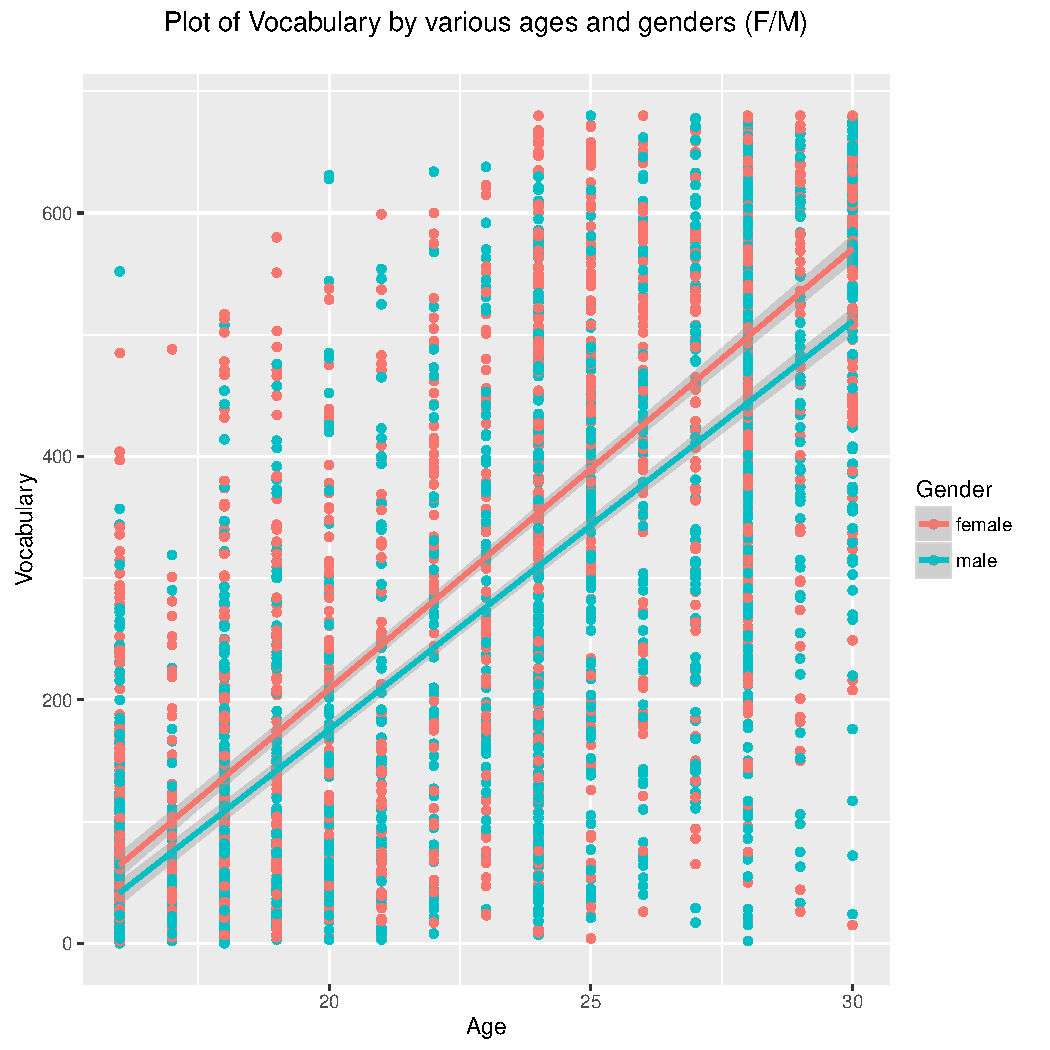
\includegraphics[width=.9\textwidth]{wordbank-age-gender.pdf}
  \caption{Linear model of ratings and age and gender.}
  \label{fig:sfig2}
\end{subfigure}
\label{fig:fig}
\end{figure}

\begin{table*}[ht]
\begin{tabular}{l*{1}{c}r}
Category & Sample Size \\
\hline
Gender& Male: 2091 Female: 1981 \\
\hline
Race & Asian: 71 Hispanic: 133 Black: 231 White: 2228 Other: 100  \\
\hline
& Graduate: 577 Some Graduate: 157 College: 850 \\
 Education & Some College: 601 Secondary: 433 \\
 & Some Secondary: 128 Primary: 8 \\
 \hline
 & First: 1423 Second: 920 Third: 284 Fourth: 92 \\
Birth Order & Fifth: 20 Sixth: 10 Seventh: 4 Eighth: 1 \\
\hline
\end{tabular}
\caption{Sample size in terms of gender and race.}
\label{tab1}
\end{table*}

To find the more detailed relationship, we perform the linear regression prediction for vocabulary size using all the variables, including age, gender, ethnicity, birth order, and mother's education level. In our first linear model, we convert all the categorical variables (gender, ethnicity, birth order, and mother's education level) into dummy variables, and use R's lm function to achieve our model. By making all the variables dummy variables, we can obtain the first model with Multiple R-squared value being 0.5151. From the model, age and gender has the lowest P values which are less than 2e-16. Small P value shows that it is more likely to fit the data. Each unit increase in age (one month) will cause 33.3164 increase in the mean value of vocabulary size. In general, male children will have a 48.6006 decrease of mean value of vocabulary size. Followed by age and gender, comes the factor of being white, or having a mother with secondary education, or college education. However, the P value for those variables are significantly larger which are around 0.0005. Thus the results shows that both birth order and graduate education level has no impact on the vocabulary size.

In order to improve the model, only age and gender were used as predictors. As the model turns out, it has a Multiple R-squared value being 0.6095 which shows that the model is better than the previous one with a Multiple R-squared value being 0.515. However, with the sample size being 5498, a maximum size of 74 predictor variables can be used, so more tests were done to see if a better model can be obtained.

A further analysis of linear model of vocabulary size using age and gender, only race, only education level, and only birth order, further proves that birth order has no impact on the vocabulary size. Specifically, the race factor, as shown in the third model with a multiple R-squared being 0.005969 which is very small. As a result, the race factor is not selected as a predictor. On the other hand, we observe the factor of being white, which has a small p value being 0.0086, and discover that the sample population is over 2000. As the sample size grows, any data can become significant, so a small p-value does not make being white or not a good predictor. Then with a model formed around the order of the child's birth, a multiple R-squared value of 0.01739 is obtained which is still rather small. For education level, it has even smaller adjusted R-squared value than birth order (0.004584 vs. 0.01488). Moreover, every single factor in this model has a P-value over 0.1 which showed that this model is not a good fit either. The linear model with all the above factors excluded and uses only age and gender achieves a highest adjusted R-squared value of 0.6093.

Based on the above reasoning, we finalize our linear model with only gender and age. The linear model is presented as follows:
\begin{align*}
\bar{V} &= b_0 + b_1 Age + b_2 IsMale \\
b_0 &= -484.1307 \\
b_1 &= 34.8168 \\
b_2 &= -39.6868 \\
IsMale &= \{1,0\} \\
\end{align*}

We conclude that age (in month) significantly predicted positive vocabulary size, $b_1=34.8168$, $t(4096)=79.239$, $p<2e-16$; gender (whether the child is male or not) significantly predicted negative vocabulary size, $b_2=-39.6868$, $t(4096)=-9.208$, $p<2e-16$. Together age and gender explained a large portion of variance in vocabulary sizes, $R^2=.6093, F(2,4096)=3176, p<2.2e-16$. One month of age growth will contribute to 34.8168 increase of vocabulary size, being a male child will contribute to 39.6868 decrease of vocabulary size.

\appendix
\section*{Appendix: Linear Model Outputs for Problem B}

\begin{lstlisting}[language=R]
## Vocab ~ Age + Gender + Race + Education + Birth Order

Residuals:
    Min      1Q  Median      3Q     Max
-464.46  -96.28   -4.51   94.00  471.77

Coefficients: (2 not defined because of singularities)
                     Estimate Std. Error t value Pr(>|t|)
(Intercept)         -583.1965   145.0625  -4.020 5.97e-05 ***
x$age                 33.3164     0.6432  51.800  < 2e-16 ***
x$is_male            -48.6006     5.4930  -8.848  < 2e-16 ***
x$is_asian            38.3629    22.7837   1.684 0.092338 .
x$is_black            54.0626    17.3605   3.114 0.001864 **
x$is_hispanic        -23.1461    19.1766  -1.207 0.227539
x$is_white            53.0242    15.3290   3.459 0.000550 ***
x$is_primary        -106.3800    51.5485  -2.064 0.039142 *
x$is_some_secondary  -49.9880    15.0552  -3.320 0.000911 ***
x$is_secondary       -21.4568     9.3609  -2.292 0.021971 *
x$is_some_college    -29.5289     8.4764  -3.484 0.000502 ***
x$is_college         -17.9607     7.7583  -2.315 0.020686 *
x$is_some_graduate    -8.1601    12.9772  -0.629 0.529532
x$is_graduate              NA         NA      NA       NA
x$is_first           115.7452   143.7341   0.805 0.420733
x$is_second           90.1358   143.7723   0.627 0.530755
x$is_third            66.9958   143.9505   0.465 0.641676
x$is_fourth           81.6032   144.4836   0.565 0.572262
x$is_fifth            40.9479   147.1721   0.278 0.780856
x$is_sixth            -2.1739   150.7379  -0.014 0.988494
x$is_seventh         -63.5342   160.6141  -0.396 0.692453
x$is_eighth                NA         NA      NA       NA
---
Signif. codes:  0 ‘***’ 0.001 ‘**’ 0.01 ‘*’
0.05 ‘.’ 0.1 ‘ ’ 1

Residual standard error: 143.2 on 2721 degrees of freedom
  (2757 observations deleted due to missingness)
Multiple R-squared:  0.5151,	Adjusted R-squared:  0.5117
F-statistic: 152.1 on 19 and 2721 DF,  p-value: < 2.2e-16
\end{lstlisting}

\begin{lstlisting}[language=R]
## Age + Gender

Call:
lm(formula = x$vocab ~ x$age + x$is_male)

Residuals:
    Min      1Q  Median      3Q     Max
-545.37  -76.50   -5.42   91.22  518.75

Coefficients:
             Estimate Std. Error t value Pr(>|t|)
(Intercept) -484.1307    10.3192 -46.915   <2e-16 ***
x$age         34.8168     0.4394  79.239   <2e-16 ***
x$is_male    -39.6868     4.3099  -9.208   <2e-16 ***
---
Signif. codes:  0 ‘***’ 0.001 ‘**’ 0.01 ‘*’
0.05 ‘.’ 0.1 ‘ ’ 1

Residual standard error: 137.5 on 4069 degrees of freedom
  (1426 observations deleted due to missingness)
Multiple R-squared:  0.6095,	Adjusted R-squared:  0.6093
F-statistic:  3176 on 2 and 4069 DF,  p-value: < 2.2e-16
\end{lstlisting}

\begin{lstlisting}[language=R]
## Race

Residuals:
    Min      1Q  Median      3Q     Max
-280.32 -191.63  -33.32  178.68  446.58

Coefficients:
              Estimate Std. Error t value Pr(>|t|)
(Intercept)    225.420     20.424  11.037   <2e-16 ***
x$is_asian      38.524     31.697   1.215   0.2243
x$is_black      58.329     24.449   2.386   0.0171 *
x$is_hispanic   -2.172     27.033  -0.080   0.9360
x$is_white      54.900     20.878   2.630   0.0086 **
---
Signif. codes:  0 ‘***’ 0.001 ‘**’ 0.01 ‘*’
0.05 ‘.’ 0.1 ‘ ’ 1

Residual standard error: 204.2 on 2758 degrees of freedom
  (2735 observations deleted due to missingness)
Multiple R-squared:  0.005969,	Adjusted R-squared:  0.004527
F-statistic:  4.14 on 4 and 2758 DF,  p-value: 0.002397

## Education

Residuals:
    Min      1Q  Median      3Q     Max
-287.14 -190.48  -36.48  178.78  433.95

Coefficients: (1 not defined because of singularities)
                     Estimate Std. Error t value Pr(>|t|)
(Intercept)          289.1352     8.5078  33.985  < 2e-16 ***
x$is_primary        -144.6352    72.7530  -1.988 0.046907 *
x$is_some_secondary  -66.0883    19.9668  -3.310 0.000945 ***
x$is_secondary        -2.9366    12.9938  -0.226 0.821219
x$is_some_college    -26.6593    11.9111  -2.238 0.025289 *
x$is_college         -12.6599    11.0235  -1.148 0.250886
x$is_some_graduate     0.4126    18.3957   0.022 0.982108
x$is_graduate              NA         NA      NA       NA
---
Signif. codes:  0 ‘***’ 0.001 ‘**’ 0.01 ‘*’
0.05 ‘.’ 0.1 ‘ ’ 1

Residual standard error: 204.4 on 2747 degrees of freedom
  (2744 observations deleted due to missingness)
Multiple R-squared:  0.006753,	Adjusted R-squared:  0.004584
F-statistic: 3.113 on 6 and 2747 DF,  p-value: 0.004842

## Birth Order

Residuals:
    Min      1Q  Median      3Q     Max
-296.44 -189.49  -33.92  175.31  454.51

Coefficients: (1 not defined because of singularities)
             Estimate Std. Error t value Pr(>|t|)
(Intercept)       4.0      203.2   0.020    0.984
x$is_first      292.4      203.3   1.438    0.150
x$is_second     260.0      203.3   1.279    0.201
x$is_third      218.5      203.6   1.073    0.283
x$is_fourth     248.7      204.3   1.217    0.224
x$is_fifth      198.9      208.2   0.955    0.339
x$is_sixth      195.4      213.1   0.917    0.359
x$is_seventh     59.5      227.2   0.262    0.793
x$is_eighth        NA         NA      NA       NA

Residual standard error: 203.2 on 2746 degrees of freedom
  (2744 observations deleted due to missingness)
Multiple R-squared:  0.01739,	Adjusted R-squared:  0.01488
F-statistic: 6.942 on 7 and 2746 DF,  p-value: 3.238e-08
\end{lstlisting}



\begin{lstlisting}[language=R]
\end{lstlisting}

\begin{lstlisting}[language=R]
\end{lstlisting}

\begin{lstlisting}[language=R]
\end{lstlisting}

\end{document}

%%
%% End of file.